\documentclass[twoside]{book}

% Packages required by doxygen
\usepackage{fixltx2e}
\usepackage{calc}
\usepackage{doxygen}
\usepackage[export]{adjustbox} % also loads graphicx
\usepackage{graphicx}
\usepackage[utf8]{inputenc}
\usepackage{makeidx}
\usepackage{multicol}
\usepackage{multirow}
\PassOptionsToPackage{warn}{textcomp}
\usepackage{textcomp}
\usepackage[nointegrals]{wasysym}
\usepackage[table]{xcolor}

% Font selection
\usepackage[T1]{fontenc}
\usepackage[scaled=.90]{helvet}
\usepackage{courier}
\usepackage{amssymb}
\usepackage{sectsty}
\renewcommand{\familydefault}{\sfdefault}
\allsectionsfont{%
  \fontseries{bc}\selectfont%
  \color{darkgray}%
}
\renewcommand{\DoxyLabelFont}{%
  \fontseries{bc}\selectfont%
  \color{darkgray}%
}
\newcommand{\+}{\discretionary{\mbox{\scriptsize$\hookleftarrow$}}{}{}}

% Page & text layout
\usepackage{geometry}
\geometry{%
  a4paper,%
  top=2.5cm,%
  bottom=2.5cm,%
  left=2.5cm,%
  right=2.5cm%
}
\tolerance=750
\hfuzz=15pt
\hbadness=750
\setlength{\emergencystretch}{15pt}
\setlength{\parindent}{0cm}
\setlength{\parskip}{3ex plus 2ex minus 2ex}
\makeatletter
\renewcommand{\paragraph}{%
  \@startsection{paragraph}{4}{0ex}{-1.0ex}{1.0ex}{%
    \normalfont\normalsize\bfseries\SS@parafont%
  }%
}
\renewcommand{\subparagraph}{%
  \@startsection{subparagraph}{5}{0ex}{-1.0ex}{1.0ex}{%
    \normalfont\normalsize\bfseries\SS@subparafont%
  }%
}
\makeatother

% Headers & footers
\usepackage{fancyhdr}
\pagestyle{fancyplain}
\fancyhead[LE]{\fancyplain{}{\bfseries\thepage}}
\fancyhead[CE]{\fancyplain{}{}}
\fancyhead[RE]{\fancyplain{}{\bfseries\leftmark}}
\fancyhead[LO]{\fancyplain{}{\bfseries\rightmark}}
\fancyhead[CO]{\fancyplain{}{}}
\fancyhead[RO]{\fancyplain{}{\bfseries\thepage}}
\fancyfoot[LE]{\fancyplain{}{}}
\fancyfoot[CE]{\fancyplain{}{}}
\fancyfoot[RE]{\fancyplain{}{\bfseries\scriptsize Generated by Doxygen }}
\fancyfoot[LO]{\fancyplain{}{\bfseries\scriptsize Generated by Doxygen }}
\fancyfoot[CO]{\fancyplain{}{}}
\fancyfoot[RO]{\fancyplain{}{}}
\renewcommand{\footrulewidth}{0.4pt}
\renewcommand{\chaptermark}[1]{%
  \markboth{#1}{}%
}
\renewcommand{\sectionmark}[1]{%
  \markright{\thesection\ #1}%
}

% Indices & bibliography
\usepackage{natbib}
\usepackage[titles]{tocloft}
\setcounter{tocdepth}{3}
\setcounter{secnumdepth}{5}
\makeindex

% Hyperlinks (required, but should be loaded last)
\usepackage{ifpdf}
\ifpdf
  \usepackage[pdftex,pagebackref=true]{hyperref}
\else
  \usepackage[ps2pdf,pagebackref=true]{hyperref}
\fi
\hypersetup{%
  colorlinks=true,%
  linkcolor=blue,%
  citecolor=blue,%
  unicode%
}

% Custom commands
\newcommand{\clearemptydoublepage}{%
  \newpage{\pagestyle{empty}\cleardoublepage}%
}

\usepackage{caption}
\captionsetup{labelsep=space,justification=centering,font={bf},singlelinecheck=off,skip=4pt,position=top}

%===== C O N T E N T S =====

\begin{document}

% Titlepage & ToC
\hypersetup{pageanchor=false,
             bookmarksnumbered=true,
             pdfencoding=unicode
            }
\pagenumbering{roman}
\begin{titlepage}
\vspace*{7cm}
\begin{center}%
{\Large My Project }\\
\vspace*{1cm}
{\large Generated by Doxygen 1.8.11}\\
\end{center}
\end{titlepage}
\clearemptydoublepage
\tableofcontents
\clearemptydoublepage
\pagenumbering{arabic}
\hypersetup{pageanchor=true}

%--- Begin generated contents ---
\chapter{File Index}
\section{File List}
Here is a list of all files with brief descriptions\+:\begin{DoxyCompactList}
\item\contentsline{section}{\hyperlink{Lab1_8c}{Lab1.\+c} }{\pageref{Lab1_8c}}{}
\end{DoxyCompactList}

\chapter{File Documentation}
\hypertarget{String_8c}{}\section{String.\+c File Reference}
\label{String_8c}\index{String.\+c@{String.\+c}}
{\ttfamily \#include $<$stdio.\+h$>$}\\*
{\ttfamily \#include $<$string.\+h$>$}\\*
{\ttfamily \#include $<$stdlib.\+h$>$}\\*
Include dependency graph for String.\+c\+:
\nopagebreak
\begin{figure}[H]
\begin{center}
\leavevmode
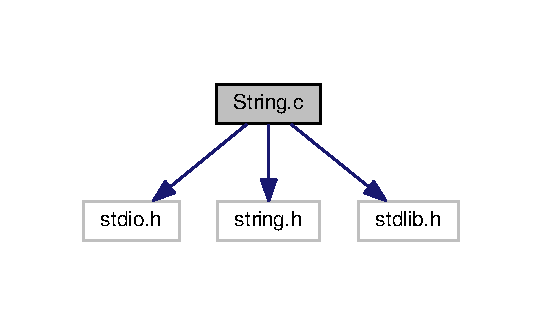
\includegraphics[width=260pt]{String_8c__incl}
\end{center}
\end{figure}
\subsection*{Macros}
\begin{DoxyCompactItemize}
\item 
\#define \hyperlink{String_8c_a0c8dad16ba61ded55d3f302a616c0ced}{M\+A\+X\+B\+U\+FF}~128
\end{DoxyCompactItemize}
\subsection*{Functions}
\begin{DoxyCompactItemize}
\item 
int \hyperlink{String_8c_a66e16d009be8c1f85a994d06a8ad8f05}{getline} (char line\mbox{[}$\,$\mbox{]}, int nmax)
\item 
int \hyperlink{String_8c_a00e28c6b7415fcf87da3e30b7e067549}{compact1} (char line\mbox{[}$\,$\mbox{]})
\item 
int \hyperlink{String_8c_a41457fd237e556dc2f67a16ca2027177}{compact2} (char line\mbox{[}$\,$\mbox{]})
\item 
int \hyperlink{String_8c_a840291bc02cba5474a4cb46a9b9566fe}{main} (void)
\end{DoxyCompactItemize}


\subsection{Macro Definition Documentation}
\index{String.\+c@{String.\+c}!M\+A\+X\+B\+U\+FF@{M\+A\+X\+B\+U\+FF}}
\index{M\+A\+X\+B\+U\+FF@{M\+A\+X\+B\+U\+FF}!String.\+c@{String.\+c}}
\subsubsection[{\texorpdfstring{M\+A\+X\+B\+U\+FF}{MAXBUFF}}]{\setlength{\rightskip}{0pt plus 5cm}\#define M\+A\+X\+B\+U\+FF~128}\hypertarget{String_8c_a0c8dad16ba61ded55d3f302a616c0ced}{}\label{String_8c_a0c8dad16ba61ded55d3f302a616c0ced}


\subsection{Function Documentation}
\index{String.\+c@{String.\+c}!compact1@{compact1}}
\index{compact1@{compact1}!String.\+c@{String.\+c}}
\subsubsection[{\texorpdfstring{compact1(char line[])}{compact1(char line[])}}]{\setlength{\rightskip}{0pt plus 5cm}int compact1 (
\begin{DoxyParamCaption}
\item[{char}]{line\mbox{[}$\,$\mbox{]}}
\end{DoxyParamCaption}
)}\hypertarget{String_8c_a00e28c6b7415fcf87da3e30b7e067549}{}\label{String_8c_a00e28c6b7415fcf87da3e30b7e067549}

\begin{DoxyCode}
51 \{
52   \textcolor{keywordtype}{int} cursor=0;      \textcolor{comment}{/* Cursor on the line */}
53   \textcolor{keywordtype}{int} prevspace = 0; \textcolor{comment}{/* True iff preceding position was with a space */}
54   \textcolor{keywordtype}{int} lcv=0;         \textcolor{comment}{/* Other cursor */}
55 
56   \textcolor{keywordflow}{if}(line[cursor]==\textcolor{charliteral}{'\(\backslash\)0'})
57     \textcolor{keywordflow}{return} 0;
58   \textcolor{keywordflow}{do}\{
59     \textcolor{keywordflow}{if}((line[cursor]==\textcolor{charliteral}{' '})&&prevspace)\{
60       \textcolor{comment}{/*If we have a space preceded by a space, move rest of string
}
61 \textcolor{comment}{    left one position */}
62       \textcolor{keywordflow}{for}(lcv=cursor;line[lcv];lcv++)
63     line[lcv]=line[lcv+1];
64     \}\textcolor{keywordflow}{else}
65       prevspace=(line[cursor++]==\textcolor{charliteral}{' '});
66   \}\textcolor{keywordflow}{while}(line[cursor]);
67   \textcolor{keywordflow}{return} cursor;
68 \}
\end{DoxyCode}
\index{String.\+c@{String.\+c}!compact2@{compact2}}
\index{compact2@{compact2}!String.\+c@{String.\+c}}
\subsubsection[{\texorpdfstring{compact2(char line[])}{compact2(char line[])}}]{\setlength{\rightskip}{0pt plus 5cm}int compact2 (
\begin{DoxyParamCaption}
\item[{char}]{line\mbox{[}$\,$\mbox{]}}
\end{DoxyParamCaption}
)}\hypertarget{String_8c_a41457fd237e556dc2f67a16ca2027177}{}\label{String_8c_a41457fd237e556dc2f67a16ca2027177}

\begin{DoxyCode}
74 \{
75   \textcolor{keywordtype}{int} cursor=0;      \textcolor{comment}{/* Cursor on the line */}
76   \textcolor{keywordtype}{int} prevspace = 0; \textcolor{comment}{/* True iff preceding position was with a space */}
77   \textcolor{keywordtype}{int} lcv = 0;       \textcolor{comment}{/* Where we copy characters to */}
78 
79   \textcolor{keywordflow}{do}\{
80     \textcolor{keywordflow}{if}(!((line[cursor]==\textcolor{charliteral}{' '})&&prevspace))\{
81       line[lcv++]=line[cursor];
82       prevspace=(line[cursor]==\textcolor{charliteral}{' '});
83     \}
84   \}\textcolor{keywordflow}{while}(line[cursor++]);
85   \textcolor{keywordflow}{return}(lcv-1); \textcolor{comment}{/*We need the -1 since it counts also the '\(\backslash\)0' */}
86 \}
\end{DoxyCode}
\index{String.\+c@{String.\+c}!getline@{getline}}
\index{getline@{getline}!String.\+c@{String.\+c}}
\subsubsection[{\texorpdfstring{getline(char line[], int nmax)}{getline(char line[], int nmax)}}]{\setlength{\rightskip}{0pt plus 5cm}int getline (
\begin{DoxyParamCaption}
\item[{char}]{line\mbox{[}$\,$\mbox{]}, }
\item[{int}]{nmax}
\end{DoxyParamCaption}
)}\hypertarget{String_8c_a66e16d009be8c1f85a994d06a8ad8f05}{}\label{String_8c_a66e16d009be8c1f85a994d06a8ad8f05}

\begin{DoxyCode}
35 \{
36   \textcolor{keywordtype}{int} len;
37   \textcolor{keywordtype}{char} c;
38 
39   len = 0;
40   printf(\textcolor{stringliteral}{"Enter a string [CR to exit]: "});
41   \textcolor{keywordflow}{while}(((c=getchar())!=\textcolor{charliteral}{'\(\backslash\)n'}) && len<nmax-1)
42     line[len++]=c;
43   line[len]=\textcolor{charliteral}{'\(\backslash\)0'};
44   \textcolor{keywordflow}{return} len;
45 \}
\end{DoxyCode}
\index{String.\+c@{String.\+c}!main@{main}}
\index{main@{main}!String.\+c@{String.\+c}}
\subsubsection[{\texorpdfstring{main(void)}{main(void)}}]{\setlength{\rightskip}{0pt plus 5cm}int main (
\begin{DoxyParamCaption}
\item[{void}]{}
\end{DoxyParamCaption}
)}\hypertarget{String_8c_a840291bc02cba5474a4cb46a9b9566fe}{}\label{String_8c_a840291bc02cba5474a4cb46a9b9566fe}

\begin{DoxyCode}
14                \{
15   \textcolor{keywordtype}{char} buffer1[\hyperlink{String_8c_a0c8dad16ba61ded55d3f302a616c0ced}{MAXBUFF}];
16   \textcolor{keywordtype}{char} buffer2[\hyperlink{String_8c_a0c8dad16ba61ded55d3f302a616c0ced}{MAXBUFF}];
17   \textcolor{keywordtype}{int} len;
18 
19   len = \hyperlink{String_8c_a66e16d009be8c1f85a994d06a8ad8f05}{getline}(buffer1, \hyperlink{String_8c_a0c8dad16ba61ded55d3f302a616c0ced}{MAXBUFF});
20   printf(\textcolor{stringliteral}{"You entered : %s\(\backslash\)n"}, buffer1);
21   strcpy(buffer2,buffer1);
22   printf(\textcolor{stringliteral}{"Which is : %s\(\backslash\)n"}, buffer2);
23 
24   len=\hyperlink{String_8c_a00e28c6b7415fcf87da3e30b7e067549}{compact1}(buffer1);
25   printf(\textcolor{stringliteral}{"compact1: len=%d,  %s\(\backslash\)n"},len, buffer1);
26   len=\hyperlink{String_8c_a41457fd237e556dc2f67a16ca2027177}{compact2}(buffer2);
27   printf(\textcolor{stringliteral}{"compact2: len=%d,  %s\(\backslash\)n"},len, buffer2);
28 \}
\end{DoxyCode}


Here is the call graph for this function\+:
\nopagebreak
\begin{figure}[H]
\begin{center}
\leavevmode
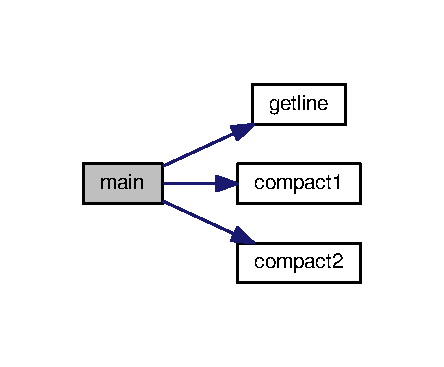
\includegraphics[width=213pt]{String_8c_a840291bc02cba5474a4cb46a9b9566fe_cgraph}
\end{center}
\end{figure}



%--- End generated contents ---

% Index
\backmatter
\newpage
\phantomsection
\clearemptydoublepage
\addcontentsline{toc}{chapter}{Index}
\printindex

\end{document}
